\PassOptionsToPackage{svgnames}{xcolor}
\documentclass[12pt,a4paper]{article}
\usepackage[utf8x]{inputenc}
\usepackage[portuguese]{babel}
\usepackage[T1]{fontenc}
\usepackage{amsmath, amssymb, amsfonts}
\usepackage{graphicx}
\usepackage{indentfirst}
\usepackage[left=2cm,right=2cm, top=4cm, bottom=2cm]{geometry}
\usepackage[colorlinks=true,allcolors=blue]{hyperref} % links 
\usepackage[table]{xcolor}
\usepackage{booktabs}
\usepackage{enumitem}
\usepackage{paralist}
\usepackage{makecell}
\usepackage{multicol}
\usepackage{multirow}
\usepackage[title]{appendix}
\usepackage{enumitem}
\usepackage{tabularx,ragged2e}
\usepackage[hang,flushmargin, bottom]{footmisc} %retira a identação da%footnote
\usepackage{adjustbox}


% to make myblock
\usepackage{tcolorbox}
\usepackage{lipsum}
\tcbuselibrary{skins,breakable}
\usetikzlibrary{shadings,shadows}

\usepackage{lipsum}
\usepackage{float}
\usepackage{graphicx,eso-pic}
\usepackage{lipsum}



\usepackage{epstopdf}
\epstopdfsetup{outdir=./}


\usepackage{longtable}
\usepackage{caption,setspace}

\captionsetup{skip=0pt}


\AddToShipoutPictureBG{%
  \AtPageUpperLeft{%
    \raisebox{-\height}{
\includegraphics[width=20cm, height=3.8cm]{figures/head2.png}}
  }
  %\AtPageLowerLeft{%
   % \makebox[\paperwidth]{\includegraphics[height=1.7cm]{figures/bottom.png}}
  %}
}

%%%%%%%%%%%% setlength

\setlength{\skip\footins}{12mm} %<------------ space between text and footnote
\setlength{\columnsep}{1cm}
\setlength{\parskip}{0pt}



%%%%%%%%%%%% New commands

\newenvironment{myexampleblock}[1]{
    \tcolorbox[
    %noparskip,
    breakable,
    colframe=blue!85!black,
    colback=white,
    title=#1]}
    {\endtcolorbox}


\newcommand{\tri}{$\blacktriangleright \:$}

\usepackage{lmodern}

\makeatletter
\ifcase \@ptsize \relax% 10pt
  \newcommand{\miniscule}{\@setfontsize\miniscule{2}{3}}% \tiny: 5/6
\or% 11pt
  \newcommand{\miniscule}{\@setfontsize\miniscule{4}{5}}% \tiny: 6/7
\or% 12pt
  \newcommand{\miniscule}{\@setfontsize\miniscule{4}{5}}% \tiny: 6/7
\fi
\makeatother


\newcolumntype{P}[1]{>{\centering\arraybackslash}p{#1}} % centralizar elementos da tabela


\graphicspath{{figures/}}


%%%%%%%%%%%%%%%%%%%%%%%%%%%%%%% Start %%%%%%%%%%%%%%%%%%%%%%%%%%%%%%%%%%%%%%%

\begin{document}

\begin{multicols}{2}

\begin{flushleft}
Luciano Nakabashi \\        
Marcos Júnio Ribeiro \\
Francielly Almeida  \\
\end{flushleft}

\begin{flushright}
Pedro Borges \\
Nícolas Volgarine Scaraboto \\
Rafael de Castro Perez \\
\end{flushright}

\end{multicols}

\vspace{0.2cm}


% sections --------------


\section{Introdução}

\begin{multicols}{2}

O saneamento básico ganhou bastante atenção de pesquisadores e governos ao longo das últimas décadas. Isso devido ao fato de estar associado a saúde, bem estar e também ao meio ambiente. O saneamento adequado pode trazer muitos benefícios a população, por exemplo: melhor nutrição, higiene pessoal, e prevenção a doenças relacionadas à água contaminada. Além disso pode haver também benefícios indiretos como aumento do comércio e crescimento econômico.

A Índia por exemplo, é o segundo país mais populoso do mundo e sofre com os problemas associados a falta saneamento básico\footnote{
Dados do \href{https://data.worldbank.org/indicator/SH.STA.BASS.ZS?locations=IN}{Banco Mundial} mostram que 71\% da população indiana possui acesso a serviços de saneamento básico. No entanto, vale ressaltar que esses dados não dizem nada a respeito da qualidade e condições desse serviço.
}. Esse fato motivou a criação, por parte do governo, do programa \href{https://siwi.org/latest/the-clean-india-mission-worlds-largest-sanitation-initiative/}{Índia limpa} em que uma das ações foi construir 100 milhões de banheiros públicos.


No Brasil, no dia 15/07/2020 foi sancionada a \href{http://www.planalto.gov.br/ccivil_03/_ato2019-2022/2020/lei/l14026.htm}{Lei $N^\circ \, 14.026$} que atualiza o marco legal do saneamento básico e altera a Lei $N^\circ \, 9.984$, de julho de 2000. O principal objetivo da Lei é universalizar e qualificar a prestação dos serviços de água e esgoto do país. 

No \href{https://www.fundace.org.br/assets/uploads/_up_ceper_estudos/ceper_20210_00035.pdf}{Boletim Saneamento} de fevereiro de 2021 mostramos que o setor de saneamento no estado de São Paulo vem se aprimorando, sobretudo no
atendimento total de água e coleta e tratamento de esgoto, mas ainda carece de melhorias\footnote{Constatamos isso também no \href{https://www.fundace.org.br/assets/uploads/_up_ceper_estudos/ceper_20210_00039.pdf}{Boletim Socioeconômico} de outubro de 2021.}. 

No presente estudo também avaliamos as condições de saneamento no estado de São Paulo. Porém, iremos considerar a natureza jurídica dos prestadores de serviços, uma vez que os governos, municipais e estaduais, para tentar atender a demanda de investimentos no setor tem adotado modelos de negócios em que a participação do capital privado é de suma importância para o sucesso do projeto.

Logo, iremos avaliar os prestadores de serviços de saneamento nos municípios paulistas utilizando quatro aspectos: custo dos serviços para o consumidor final, universalização dos serviços, desempenho financeiro e produtividade e despesas.

Para cumprir nossos objetivos, na seção \ref{s2} analisamos a natureza jurídica dos prestadores de serviços de saneamento nos municípios paulistas. Na seção \ref{s3} apresentamos os índices utilizados na nossa análise e a metodologia utilizada no estudo.



\end{multicols}





  



\section{Panorama dos investimentos em saneamento nos municípios paulistas}\label{s:panor}





\section{Resultados}\label{s4}




\begin{figure}[H]
        \centering
        	\begin{minipage}{0.55\textwidth}	
                \caption{Correlograma dos índices utilizados no estudo}
                \label{f:corr}
                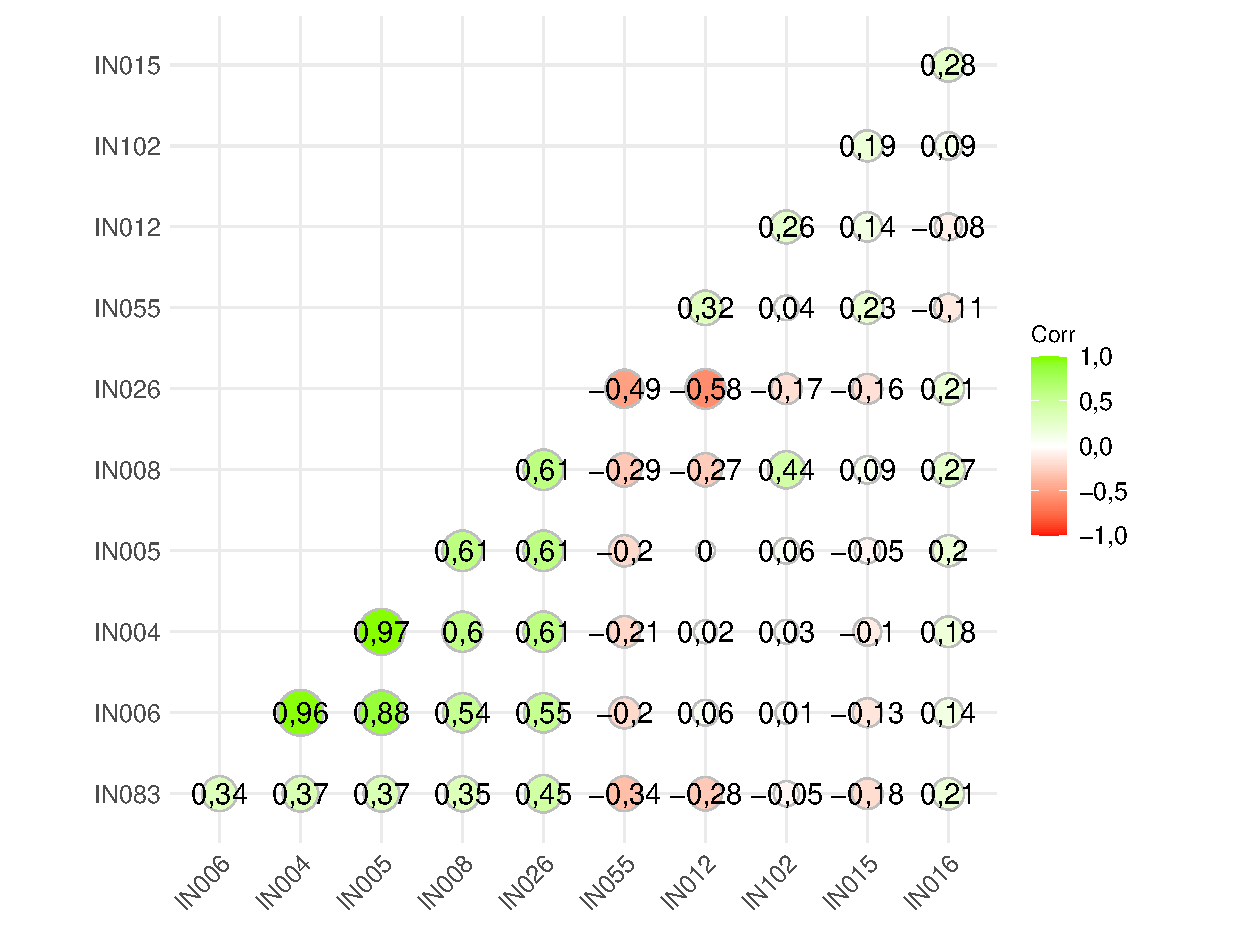
\includegraphics[scale=0.5]{corr.eps}                 
            	\footnotesize \\
            		Fonte: Elaborado pelos autores com dados do SNIS.    	
	\end{minipage}
\end{figure}







\begin{table}[H] \centering 
\begin{minipage}{1\textwidth}
  \caption{Estatístiscas descritivas dos indicadores utilizados - 2019} 
  \label{tab:desc1} 
  \tiny
    \resizebox{\textwidth}{!}{%
\begin{tabular}{@{\extracolsep{5pt}} cccccc} 
\toprule
\toprule
Índice & Média & Mediana & Máximo & Mínimo & Desvio Padrão \\ 

\midrule

IN004 & $2,50$ & $2,58$ & $4,38$ & $0,93$ & $0,98$ \\ 
IN005 & $2,67$ & $2,77$ & $4,80$ & $1,17$ & $0,93$ \\ 
IN006 & $2,30$ & $2,40$ & $3,68$ & $0,64$ & $1,08$ \\ 
\hline
IN015 & $82,89$ & $86,05$ & $100$ & $50,89$ & $14,70$ \\ 
IN016 & $86,87$ & $100$ & $100$ & $0$ & $30,75$ \\ 
IN055 & $94,75$ & $97,76$ & $100$ & $73,27$ & $6,56$ \\ 
\hline
IN012 & $91,79$ & $88,73$ & $177,52$ & $53,08$ & $26,03$ \\ 
IN102 & $415,32$ & $324,68$ & $1762,47$ & $82,66$ & $309,15$ \\ 
IN083 & $59,97$ & $2,50$ & $420,19$ & $0$ & $93,71$ \\ 
\hline
IN008 & $103.109,40$ & $70.029,21$ & $263.128,60$ & $21.148,81$ & $69.600,69$ \\ 
IN026 & $2,36$ & $2,24$ & $5,46$ & $0,66$ & $1,00$ \\ 

\bottomrule
\end{tabular} }
\footnotesize \\
	Fonte: Elaborado pelos autores com dados do SNIS. \\
	Notas: IN004 - Tarifa média praticada,
	IN005 - Tarifa média água,
	IN006 - Tarifa média esgoto,		
	IN015 - Índice de coleta de esgoto,
	IN016 - Índice de tratamento de esgoto,
	IN055 - Índice de atendimento total de água,	
	IN012 - Indicador de desempenho financeiro,
	IN102 - Índice de produtividade de pessoal total,
	IN083 - Duração média dos serviços executados,	
	IN008 - Despesa média anual por empregado,
	IN026 - Despesa de exploração por m3 faturado.
\end{minipage}
\end{table} 















\begin{table}[H] \centering 
\begin{minipage}{0.9\textwidth}
  \caption{Média dos índices - 2019} 
  \label{tab:desc2} 
  \resizebox{\textwidth}{!}{%
\begin{tabular}{@{\extracolsep{5pt}} cccccccc} 
\toprule
\toprule
Índice & \shortstack{Adm. pública \\ direta} & Autarquia & \shortstack{Empresa \\ privada} & \shortstack{Empresa \\ pública} & Mista & \shortstack{Valor Máximo} & Ranking \\ 

\midrule
 
IN004 & $1,41$ & $2,28$ & $2,79$ & $3,40$ & $3,17$ & $3,40$ & Empresa pública \\ 
IN005 & $1,49$ & $2,36$ & $2,99$ & $3,62$ & $3,37$ & $3,62$ & Empresa pública \\ 
IN006 & $0,94$ & $2,17$ & $2,57$ & $3,18$ & $2,94$ & $3,18$ & Empresa pública \\ 
IN015 & $81,50$ & $86,31$ & $84,78$ & $98$ & $86,50$ & $98$ & Empresa pública \\ 
IN016 & $74,89$ & $77,98$ & $79,90$ & $79,06$ & $94,55$ & $94,55$ & Mista \\ 
IN055 & $90,81$ & $95,99$ & $94,34$ & $94,14$ & $85,23$ & $95,99$ & Autarquia \\ 
IN012 & $99,63$ & $104,99$ & $110,53$ & $100,94$ & $93,19$ & $110,53$ & Empresa privada \\ 
IN102 & $554,23$ & $306,31$ & $388,25$ & $263,98$ & $715,59$ & $715,59$ & Mista \\ 
IN083 & $4,23$ & $7,44$ & $6,47$ & $0,62$ & $70,15$ & $70,15$ & Mista \\ 
IN008 & $43.690,26$ & $62.242,77$ & $64.024,46$ & $95.651,97$ & $215.212,00$ & $215.212,00$ & Mista \\ 
IN026 & $1,44$ & $2,06$ & $2,02$ & $3,44$ & $2,91$ & $3,44$ & Empresa pública \\

\bottomrule
\end{tabular} }
\footnotesize \\
	Fonte: Elaborado pelos autores com dados do SNIS. 
\end{minipage}
\end{table} 


\begin{table}[H] \centering 

\begin{minipage}{0.75\textwidth}
  \caption{Teste de Kruskal-Wallis nos índices utilizados na pesquisa} 
  \label{tab:krusk} 

\begin{tabular}{P{3.8cm}P{3.8cm}P{3.8cm}}
\toprule
\toprule
Índices & Valor p  do teste & H0 \\ 

\midrule

IN004 & $0,00$ & Rejeita \\ 
IN005 & $0,00$ & Rejeita \\ 
IN006 & $0,00$ & Rejeita \\ 
\hline
IN015 & $0,08$ & Rejeita \\ 
IN016 & $0,00$ & Rejeita \\ 
IN055 & $0,45$ & Aceita \\ 
\hline
IN012 & $0,42$ & Aceita \\ 
IN102 & $0,49$ & Aceita \\ 
IN083 & $0,06$ & Rejeita \\ 
\hline
IN008 & $0,49$ & Aceita \\ 
IN026 & $0,00$ & Rejeita \\ 

\bottomrule

\end{tabular} 
	\footnotesize \\
		Fonte: Elaborado pelos autores. \\ 
		Nota: A hipótese nula (H0) é de que os valores dos fazem parte da mesma população quando consideramos as diferentes naturezas jurídicas. \\
				IN004 - Tarifa média praticada,
				IN005 - Tarifa média água,
				IN006 - Tarifa média esgoto,		
				IN015 - Índice de coleta de esgoto,
				IN016 - Índice de tratamento de esgoto,
				IN055 - Índice de atendimento total de água,	
				IN012 - Indicador de desempenho financeiro,
				IN102 - Índice de produtividade de pessoal total,
				IN083 - Duração média dos serviços executados,	
				IN008 - Despesa média anual por empregado,
				IN026 - Despesa de exploração por m3 faturado.   	
\end{minipage}
\end{table} 


\begin{table}[H] \centering 
\begin{minipage}{1\textwidth}
  \caption{Coeficientes angulares das regressões estimadas para cada índice} 
  \label{tab:reg} 
  \small
  \resizebox{\textwidth}{!}{%
\begin{tabular}{ P{2.2cm}P{2.2cm}P{2.2cm}P{2.2cm}P{2.2cm}P{2.2cm} } 
\\[-1.8ex]\hline 
\hline \\[-1.8ex] 
\shortstack{Variáveis \\ independentes} & \shortstack{Adm. pública \\ direta} & Autarquia & \shortstack{Empresa \\ privada} & \shortstack{Empresa \\ pública} & Mista \\ 
\hline \\[-1.8ex] 
IN015 & $0,0084$ & $0,0009$ & $-0,0086$ & $0,4500$ & $-0,0109^{***}$ \\ 
IN016 & $-0,0006$ & $0,0029$ & $0,0039$ & $-0,0430$ & $-0,0077^{**}$ \\ 
IN055 & $-0,0246^{***}$ & $0,0096$ & $-0,0251$ & $-0,1536$ & $0,0001$ \\ 
\hline
IN012 & $0,0065^{***}$ & $0,0093^{*}$ & $-0,0008$ & $-0,0420$ & $0,0055^{**}$ \\ 
IN102 & $-0,0003^{*}$ & $-0,0015^{**}$ & $0,0002$ & $-0,0102$ & $-0,0005^{**}$ \\ 
IN083 & $0,0095$ & $0,0094$ & $0,0014$ & $7,5000$ & $0,0008$ \\ 
\hline
IN008 & $3,42e-6$ & $1,8e-5^{***}$ & $9,04e-6$ & $2,52e-5$ & $7,28e-8$ \\ 
IN026 & $0,9468^{***}$ & $0,8929^{***}$ & $0,4473^{***}$ & $0,6122^{**}$ & $0,0289$ \\ 
\hline \\[-1.8ex] 
\end{tabular} }
\footnotesize \\
	Fonte: Elaborado pelos autores com dados do SNIS. \\
	Notas: IN004 - Tarifa média praticada,
	IN005 - Tarifa média água,
	IN006 - Tarifa média esgoto,		
	IN015 - Índice de coleta de esgoto,
	IN016 - Índice de tratamento de esgoto,
	IN055 - Índice de atendimento total de água,	
	IN012 - Indicador de desempenho financeiro,
	IN102 - Índice de produtividade de pessoal total,
	IN083 - Duração média dos serviços executados,	
	IN008 - Despesa média anual por empregado,
	IN026 - Despesa de exploração por m3 faturado. \\
	Variável dependente: IN004 - Tarifa média praticada. \\
	Asteriscos simples $(*)$, duplo $(**)$ e triplo $(***)$ denotam significância a 1\%, 5\% e 10\% respectivamente. 
\end{minipage}
\end{table} 








\section{Metodologia}\label{s:metod}


\begin{multicols}{2}
Nesse boletim, analisamos quatro aspectos dos prestadores de serviços de saneamento nos municípios paulistas, considerando a natureza jurídica do prestador. São eles: custos dos serviços para o consumidor final, universalização dos serviços, desempenho financeiro e produtividade, e despesas. Para cada um desses aspectos utilizamos um conjunto de variáveis que refletem cada aspecto que queremos avaliar, isso pode ser visto na Tabela \ref{tab:ind}.
\end{multicols}




\begin{table}[H]\centering
\begin{minipage}{1\textwidth}
	\caption{Índicadores utilizados na análise}
	\label{tab:ind}
	\small
    \resizebox{\textwidth}{!}{%	
	\begin{tabular}{l|c}
		\toprule
		\toprule
			Índice & Propósito  \\
			
		\midrule
				IN004 - Tarifa média praticada  &  \multirow{3}{*}{\parbox{6cm}{Verificar o custo dos serviços para o consumidor final}} \\
				IN005 - Tarifa média água       &  \\
				IN006 - Tarifa média esgoto	   &   \\
					                                
		\midrule
				IN015 - Índice de coleta de esgoto & \multirow{3}{*}{\parbox{6cm}{Avaliar a universalização dos serviços de água e esgoto}} \\
				IN016 - Índice de tratamento de esgoto & \\
				IN055 - Índice de atendimento total de água	& \\
													
		\midrule
		
		IN012 - Indicador de desempenho financeiro & \multirow{3}{*}{\parbox{6cm}{Avaliar o desempenho financeiro e a produtividade}} \\
		IN102 - Índice de produtividade de pessoal total & \\		
		IN083 - Duração média dos serviços executados & \\
				
		\midrule
		
		IN008 - Despesa média anual por empregado & \multirow{2}{*}{\parbox{6cm}{Analisar as despesas}} \\
		IN026 - Despesa de exploração por m3 faturado & \\	
		
		\bottomrule
		
	\end{tabular} }
\footnotesize \\
	Fonte: Elaborado pelos autores.
\end{minipage}
\end{table}

\begin{multicols}{2}
Para comparar os prestadores de serviços considerando a natureza jurídica utilizamos o Teste de Kruskall-Wallis,  análise de correlação, estatísticas descritivas (média, mediana, máximo, mínimo e desvio padrão) e análise de regressão dos índices apresentados na Tabela \ref{tab:ind}.

O  Teste de Kruskall-Wallis é um teste estatístico não paramétrico utilizado para verificar se amostras de diferentes grupos fazem parte de uma mesma população.
A ideia é verificar se os valores de um determinado índice é diferente quando o agrupamos pela natureza jurídica do prestador de serviço. A hipótese nula é de que os valores de um determinado índice quando agrupados pela natureza jurídica do prestador de serviços fazem parte de uma mesma população. Caso seja aceita podemos dizer que não há diferença entre os grupos em um determinado índice.

Na análise de regressão iremos estimar a seguinte equação:
\begin{equation*}
	\text{IN004} = \alpha_0 +
	 \alpha_1 I_{j} +
	 \sum_{i=1}^{4} \beta_i N_i + 
	 \sum_{i=1}^{4} \gamma_i (N_i \times I_j)
\end{equation*}
onde $\alpha_0$ é o intercepto, $I_j$ é um dos índices da Tabela \ref{tab:ind}, sendo que $j \, \exists \, (1, 2, \cdots, 8)$, e $N_i$ é uma \textit{dummy} que indica a natureza jurídica do prestador de serviços e $i \, \exists \, (1, 2, 3, 4)$. Logo, serão estimadas oito regressões, uma para cada índice da Tabela \ref{tab:ind}, exceto para o IN005 e IN006. 

O intuito é verificar se os prestadores de serviços conseguem reduzir a tarifa média praticada (IN004) dado um aumento na universalização dos serviços, produtividade e despesas. Portanto, na nossa análise iremos focar no coeficiente angular $(\alpha_1 + \gamma_i)$. 

\end{multicols}













 

\section{Resultados}\label{s:resul}

\begin{multicols}{2}

Na Tabela \ref{tab:krusk} apresentamos o Teste de Kruskal-Wallis dos índices que analisamos. A hipótese nula $(H0)$ do teste é de que os valores de um índice específico quando agrupados pela natureza jurídica do prestador de serviços fazem parte de uma mesma população. Nota-se que somente em quatro índice rejeitamos $H0$, ou seja, para esses índices, os grupos fazem parte de populações idênticas não havendo diferenças significativas entre os prestadores de serviços.

\end{multicols}




\begin{table}[H] \centering 

\begin{minipage}{0.75\textwidth}
  \caption{Teste de Kruskal-Wallis nos índices utilizados na pesquisa} 
  \label{tab:krusk} 

\begin{tabular}{P{3.8cm}P{3.8cm}P{3.8cm}}
\toprule
\toprule
Índices & Valor p  do teste & H0 \\ 

\midrule

IN004 & $0,00$ & Rejeita \\ 
IN005 & $0,00$ & Rejeita \\ 
IN006 & $0,00$ & Rejeita \\ 
\hline
IN015 & $0,08$ & Rejeita \\ 
IN016 & $0,00$ & Rejeita \\ 
IN055 & $0,45$ & Aceita \\ 
\hline
IN012 & $0,42$ & Aceita \\ 
IN102 & $0,49$ & Aceita \\ 
IN083 & $0,06$ & Rejeita \\ 
\hline
IN008 & $0,49$ & Aceita \\ 
IN026 & $0,00$ & Rejeita \\ 

\bottomrule

\end{tabular} 
	\footnotesize \\
		Fonte: Elaborado pelos autores. \\ 
		Nota: A hipótese nula (H0) é de que os valores dos fazem parte da mesma população quando consideramos as diferentes naturezas jurídicas. \\
				IN004 - Tarifa média praticada,
				IN005 - Tarifa média água,
				IN006 - Tarifa média esgoto,		
				IN015 - Índice de coleta de esgoto,
				IN016 - Índice de tratamento de esgoto,
				IN055 - Índice de atendimento total de água,	
				IN012 - Indicador de desempenho financeiro,
				IN102 - Índice de produtividade de pessoal total,
				IN083 - Duração média dos serviços executados,	
				IN008 - Despesa média anual por empregado,
				IN026 - Despesa de exploração por m3 faturado.   	
\end{minipage}
\end{table} 


\begin{multicols}{2}

Na Figura \ref{f:corr} temos um correlograma dos índices que estamos analisando. Primeiro vamos discutir as correlações positivas e em seguida as negativas.

Nota-se que as variáveis relacionadas a tarifa média (IN004, IN005, IN006) possuem alta correlação positiva entre si, como já era de se esperar. Os índices relacionados as despesas IN008 e IN026 também possuem alta correlação positiva entre si e com os índices de despesas. Isso indica que quanto maiores as despesas, maior tende a ser as tarifas médias praticadas. 


\end{multicols}


\begin{figure}[H]
        \centering
        	\begin{minipage}{0.55\textwidth}	
                \caption{Correlograma dos índices utilizados no estudo}
                \label{f:corr}
                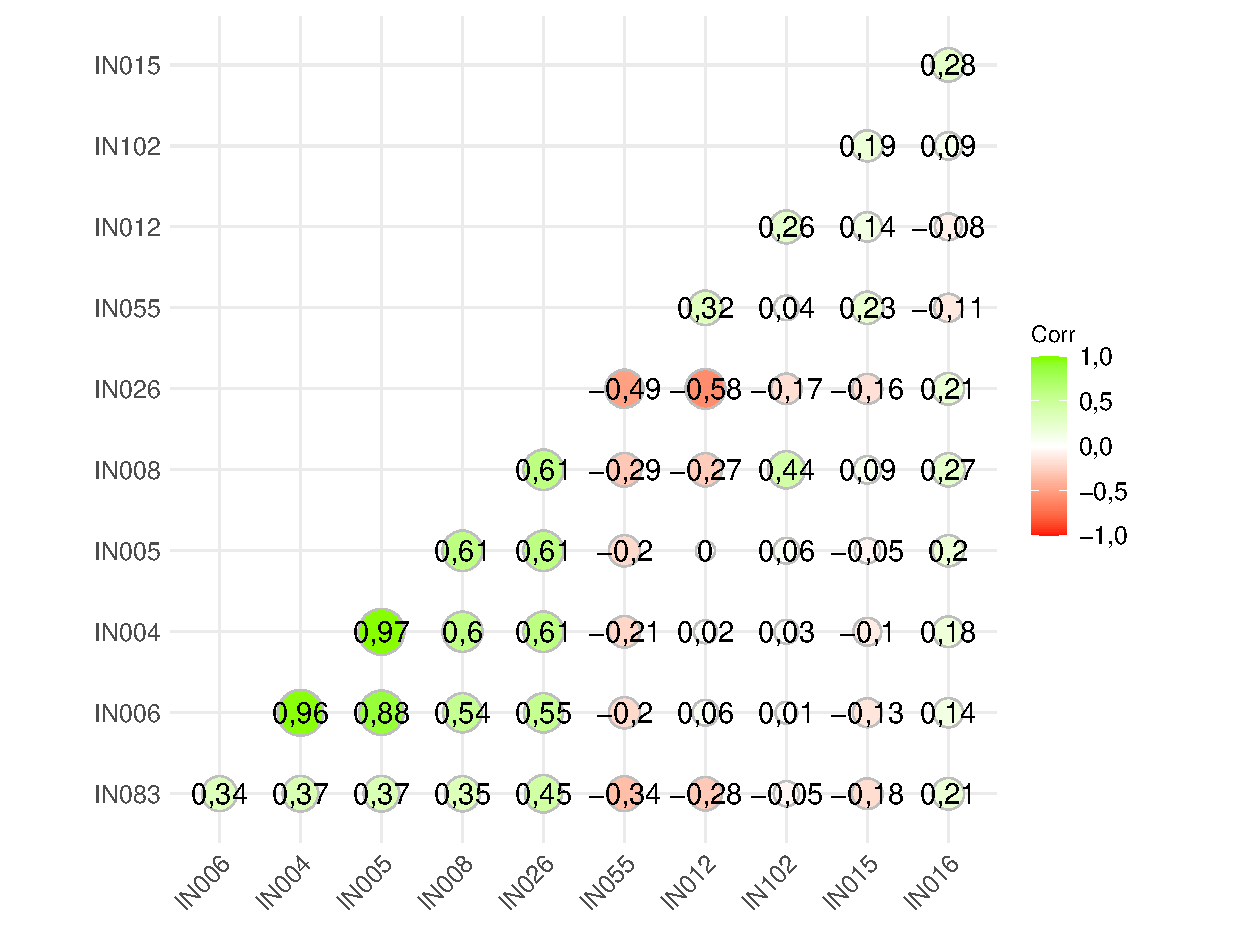
\includegraphics[scale=0.5]{figures/cor.eps}                 
            	\footnotesize \\
            		Fonte: Elaborado pelos autores com dados do SNIS. \\
            		Notas: IN004 - Tarifa média praticada,
				IN005 - Tarifa média água,
				IN006 - Tarifa média esgoto,		
				IN015 - Índice de coleta de esgoto,
				IN016 - Índice de tratamento de esgoto,
				IN055 - Índice de atendimento total de água,	
				IN012 - Indicador de desempenho financeiro,
				IN102 - Índice de produtividade de pessoal total a produtividade,
				IN083 - Duração média dos serviços executados,	
				IN008 - Despesa média anual por empregado,
				IN026 - Despesa de exploração por m3 faturado.   	
	\end{minipage}
\end{figure}







\begin{table}[H] \centering 
\begin{minipage}{1\textwidth}
  \caption{Estatístiscas descritivas dos indicadores utilizados - 2019} 
  \label{tab:desc1} 
  \tiny
    \resizebox{\textwidth}{!}{%
\begin{tabular}{@{\extracolsep{5pt}} cccccc} 
\toprule
\toprule
Índice & Média & Mediana & Máximo & Mínimo & Desvio Padrão \\ 

\midrule

IN004 & $2,50$ & $2,58$ & $4,38$ & $0,93$ & $0,98$ \\ 
IN005 & $2,67$ & $2,77$ & $4,80$ & $1,17$ & $0,93$ \\ 
IN006 & $2,30$ & $2,40$ & $3,68$ & $0,64$ & $1,08$ \\ 
\hline
IN015 & $82,89$ & $86,05$ & $100$ & $50,89$ & $14,70$ \\ 
IN016 & $86,87$ & $100$ & $100$ & $0$ & $30,75$ \\ 
IN055 & $94,75$ & $97,76$ & $100$ & $73,27$ & $6,56$ \\ 
\hline
IN012 & $91,79$ & $88,73$ & $177,52$ & $53,08$ & $26,03$ \\ 
IN102 & $415,32$ & $324,68$ & $1762,47$ & $82,66$ & $309,15$ \\ 
IN083 & $59,97$ & $2,50$ & $420,19$ & $0$ & $93,71$ \\ 
\hline
IN008 & $103.109,40$ & $70.029,21$ & $263.128,60$ & $21.148,81$ & $69.600,69$ \\ 
IN026 & $2,36$ & $2,24$ & $5,46$ & $0,66$ & $1,00$ \\ 

\bottomrule
\end{tabular} }
\footnotesize \\
	Fonte: Elaborado pelos autores com dados do SNIS. \\
	Notas: IN004 - Tarifa média praticada,
	IN005 - Tarifa média água,
	IN006 - Tarifa média esgoto,		
	IN015 - Índice de coleta de esgoto,
	IN016 - Índice de tratamento de esgoto,
	IN055 - Índice de atendimento total de água,	
	IN012 - Indicador de desempenho financeiro,
	IN102 - Índice de produtividade de pessoal total,
	IN083 - Duração média dos serviços executados,	
	IN008 - Despesa média anual por empregado,
	IN026 - Despesa de exploração por m3 faturado.
\end{minipage}
\end{table} 















\begin{table}[H] \centering 
\begin{minipage}{0.9\textwidth}
  \caption{Média dos índices - 2019} 
  \label{tab:desc2} 
  \resizebox{\textwidth}{!}{%
\begin{tabular}{@{\extracolsep{5pt}} cccccccc} 
\toprule
\toprule
Índice & \shortstack{Adm. pública \\ direta} & Autarquia & \shortstack{Empresa \\ privada} & \shortstack{Empresa \\ pública} & Mista & \shortstack{Valor Máximo} & Ranking \\ 

\midrule
 
IN004 & $1,41$ & $2,28$ & $2,79$ & $3,40$ & $3,17$ & $3,40$ & Empresa pública \\ 
IN005 & $1,49$ & $2,36$ & $2,99$ & $3,62$ & $3,37$ & $3,62$ & Empresa pública \\ 
IN006 & $0,94$ & $2,17$ & $2,57$ & $3,18$ & $2,94$ & $3,18$ & Empresa pública \\ 
IN015 & $81,50$ & $86,31$ & $84,78$ & $98$ & $86,50$ & $98$ & Empresa pública \\ 
IN016 & $74,89$ & $77,98$ & $79,90$ & $79,06$ & $94,55$ & $94,55$ & Mista \\ 
IN055 & $90,81$ & $95,99$ & $94,34$ & $94,14$ & $85,23$ & $95,99$ & Autarquia \\ 
IN012 & $99,63$ & $104,99$ & $110,53$ & $100,94$ & $93,19$ & $110,53$ & Empresa privada \\ 
IN102 & $554,23$ & $306,31$ & $388,25$ & $263,98$ & $715,59$ & $715,59$ & Mista \\ 
IN083 & $4,23$ & $7,44$ & $6,47$ & $0,62$ & $70,15$ & $70,15$ & Mista \\ 
IN008 & $43.690,26$ & $62.242,77$ & $64.024,46$ & $95.651,97$ & $215.212,00$ & $215.212,00$ & Mista \\ 
IN026 & $1,44$ & $2,06$ & $2,02$ & $3,44$ & $2,91$ & $3,44$ & Empresa pública \\

\bottomrule
\end{tabular} }
\footnotesize \\
	Fonte: Elaborado pelos autores com dados do SNIS. 
\end{minipage}
\end{table} 



\begin{table}[H] \centering 
\begin{minipage}{1\textwidth}
  \caption{Coeficientes angulares das regressões estimadas para cada índice} 
  \label{tab:reg} 
  \small
  \resizebox{\textwidth}{!}{%
\begin{tabular}{ P{2.2cm}P{2.2cm}P{2.2cm}P{2.2cm}P{2.2cm}P{2.2cm} } 
\\[-1.8ex]\hline 
\hline \\[-1.8ex] 
\shortstack{Variáveis \\ independentes} & \shortstack{Adm. pública \\ direta} & Autarquia & \shortstack{Empresa \\ privada} & \shortstack{Empresa \\ pública} & Mista \\ 
\hline \\[-1.8ex] 
IN015 & $0,0084$ & $0,0009$ & $-0,0086$ & $0,4500$ & $-0,0109^{***}$ \\ 
IN016 & $-0,0006$ & $0,0029$ & $0,0039$ & $-0,0430$ & $-0,0077^{**}$ \\ 
IN055 & $-0,0246^{***}$ & $0,0096$ & $-0,0251$ & $-0,1536$ & $0,0001$ \\ 
\hline
IN012 & $0,0065^{***}$ & $0,0093^{*}$ & $-0,0008$ & $-0,0420$ & $0,0055^{**}$ \\ 
IN102 & $-0,0003^{*}$ & $-0,0015^{**}$ & $0,0002$ & $-0,0102$ & $-0,0005^{**}$ \\ 
IN083 & $0,0095$ & $0,0094$ & $0,0014$ & $7,5000$ & $0,0008$ \\ 
\hline
IN008 & $3,42e-6$ & $1,8e-5^{***}$ & $9,04e-6$ & $2,52e-5$ & $7,28e-8$ \\ 
IN026 & $0,9468^{***}$ & $0,8929^{***}$ & $0,4473^{***}$ & $0,6122^{**}$ & $0,0289$ \\ 
\hline \\[-1.8ex] 
\end{tabular} }
\footnotesize \\
	Fonte: Elaborado pelos autores com dados do SNIS. \\
	Notas: IN004 - Tarifa média praticada,
	IN005 - Tarifa média água,
	IN006 - Tarifa média esgoto,		
	IN015 - Índice de coleta de esgoto,
	IN016 - Índice de tratamento de esgoto,
	IN055 - Índice de atendimento total de água,	
	IN012 - Indicador de desempenho financeiro,
	IN102 - Índice de produtividade de pessoal total,
	IN083 - Duração média dos serviços executados,	
	IN008 - Despesa média anual por empregado,
	IN026 - Despesa de exploração por m3 faturado. \\
	Variável dependente: IN004 - Tarifa média praticada. \\
	Asteriscos simples $(*)$, duplo $(**)$ e triplo $(***)$ denotam significância a 1\%, 5\% e 10\% respectivamente. 
\end{minipage}
\end{table} 








\section{Conclusão}\label{s:concl}


\begin{appendices}
\setcounter{table}{0}
\setcounter{figure}{0}

\renewcommand{\thetable}{A\arabic{table}}
\renewcommand{\thefigure}{A\arabic{figure}}

\section{}\label{ap1}

\begin{figure}[H]
        \centering
        	\begin{minipage}{0.8\textwidth}	
                \caption{Rigiões Administrativas do estado de São Paulo}
                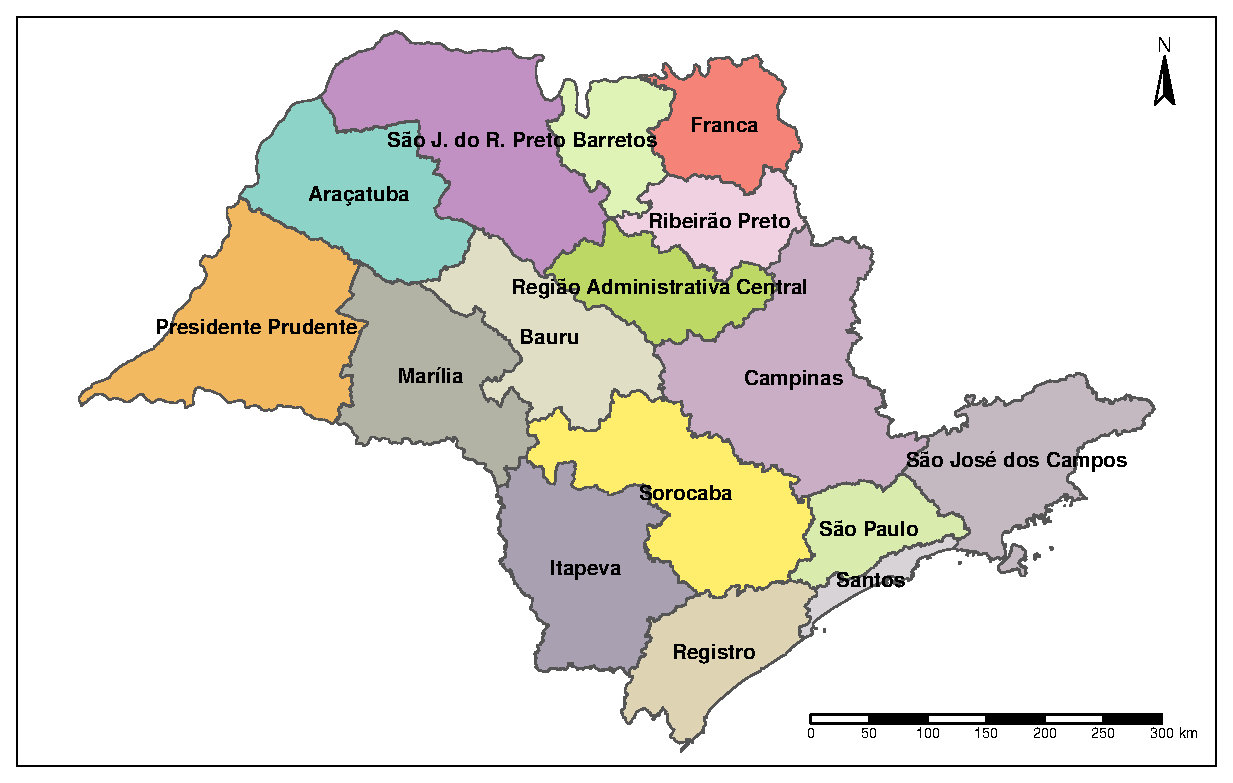
\includegraphics[scale=0.6]{figures/m2.eps}                 
            	\footnotesize \\
            		Fonte: Elaborado pelos autores.
    	\label{f:maps2}
	\end{minipage}
\end{figure}

\end{appendices}




\end{document}


